\documentclass[a4paper,11pt,exos]{nsi} % COMPILE WITH DRAFT


\pagestyle{empty}
\begin{document}

%Exercice 1E11-2



\classe{\premiere spé}
\titre{Ceinture orange 02 - Corrigé}
\maketitle

\begin{exercice}[ : Résoudre une inéquation du second degré]
    Résoudre dans $\R$ les inéquations suivantes :
    \begin{multicols}{2}
        \begin{enumerate}
            \item $-3x^2-12x-17< 0$
	        \item $2x^2-8x-10\leq 0$
	        %\item $-x^2-2x-3\leq 0$
        \end{enumerate}
    \end{multicols}
    
\end{exercice}

\begin{enumerate}
    \item Soit $P$ le polynôme défini pour tout $x$ de $\mathbb R$ par $P(x)=-3x^2-12x-17$.\\On cherche à résoudre $P(x)< 0$.\\Pour cela, on cherche ses racines éventuelles.\\$\Delta = (-12)^2-4\times(-3)\times(-17)=-60$\\$\Delta<0$ donc le polynôme $P$ n'admet pas de racine.\\ Il est toujours du signe de $a=-3<0$, donc $P(x)<0$ pour tout $x$ de $\mathbb{R}$.\\ On en déduit $S=\mathbb{R}$.
\item Soit $P$ le polynôme défini pour tout $x$ de $\mathbb R$ par $P(x)=2x^2-8x-10$.\\On cherche à résoudre $P(x)\leq 0$.\\Pour cela, on cherche ses racines éventuelles.\\$\Delta = (-8)^2-4\times2\times(-10)=144$\\$\Delta>0$ donc  le polynôme admet deux racines : $x_1 = \dfrac{-b-\sqrt{\Delta}}{2a}$ et $x_2 = \dfrac{-b+\sqrt{\Delta}}{2a}$.\\$x_1 =\dfrac{8-\sqrt{144}}{4}=-1$\\$x_2 =\dfrac{8+\sqrt{144}}{4}=5$\\On sait qu'un polynôme du second degré est du signe de $a$ à l'extérieur de ses racines.\\Comme $a=2>0 :$\\On peut résumer le signe du polynôme dans un tableau de signes :\\[.5em]
\begin{tikzpicture}[baseline, scale=0.5]
    \tkzTabInit[lgt=8,deltacl=0.8,espcl=5]{ $x$ / 2, $2x^2-8x-10$ / 2}{ $-\infty$, $-1$, $5$, $+\infty$}
	\tkzTabLine{  , +, z, -, z, +}
	\end{tikzpicture}
\\ 

Finalement $S=[-1;5]$.    
%\item Soit $P$ le polynôme défini pour tout $x$ de $\mathbb R$ par $P(x)=-x^2-2x-3$.\\On cherche à résoudre $P(x)\leq 0$.\\Pour cela, on cherche ses racines éventuelles.\\$\Delta = (-2)^2-4\times(-1)\times(-3)=-8$\\$\Delta<0$ donc le polynôme $P$ n'admet pas de racine.\\ Il est toujours du signe de $a=-1<0$, donc $P(x)<0$ pour tout $x$ de $\mathbb{R}$.\\ On en déduit $S=\mathbb{R}$.
\end{enumerate}


\end{document}